\textbf{COLUNI 2020 -- Questão 26}\par\medskip Leia os fragmentos dos textos 1 e 2 a seguir.

\par

\textbf{Texto 1}

\par

“Vi num sonho uma tabela em que todos os elementos se encaixavam como requerido. Ao despertar, escrevi-a imediatamente numa folha de papel.”

\par

Fonte: STRATHERN, Paul. \textbf{O sonho de Mendeleiev}: a verdadeira história da química. Rio de Janeiro: Jorge Zahar Ed., 2002, p. 246.

% COLUNI-AUTO-FIGURES-BEGIN
\begin{figure}[htbp]
\centering
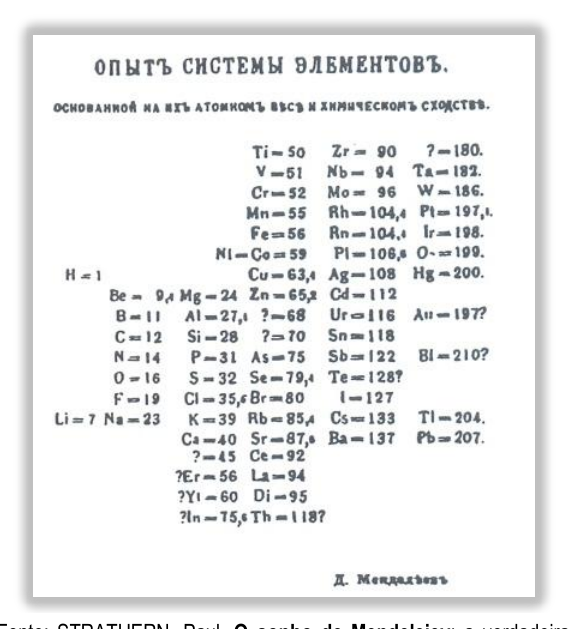
\includegraphics[width=0.95\linewidth]{static/simulados/coluni/figuras/2020/questao-26/figura-1.png}
\end{figure}
% COLUNI-AUTO-FIGURES-END

\par

Fonte: STRATHERN, Paul. \textbf{O sonho de Mendeleiev}: a verdadeira história da química. Rio de Janeiro: Jorge Zahar Ed., 2002, p. 247.

\par

\textbf{Texto 2}

% COLUNI-AUTO-FIGURES-BEGIN
\begin{figure}[htbp]
\centering
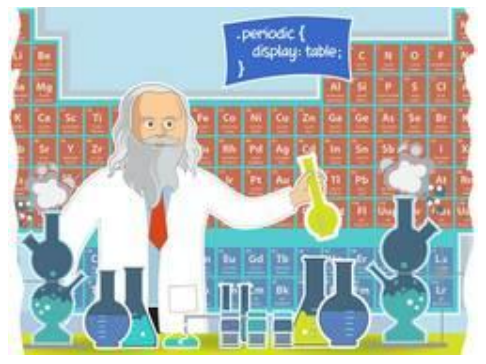
\includegraphics[width=0.95\linewidth]{static/simulados/coluni/figuras/2020/questao-26/figura-2.png}
\end{figure}
% COLUNI-AUTO-FIGURES-END

\par

A Assembleia Geral das Nações Unidas proclamou o ano de 2019 como o Ano Internacional da Tabela Periódica dos Elementos Químicos (International Year of the Periodic Table of Chemical Elements – IYPT 2019). [...] O ano de 1869 é considerado o ano da descoberta do Sistema Periódico, pelo cientista russo Dmitri Mendeleev. O IYPT 2019 também comemora os 150 anos do estabelecimento da Tabela Periódica dos Elementos Químicos.

\par

Disponível em: http://www.unesco.org/new/pt/brasilia/about-this-office/prizes-and-celebrations/2019-international-year-of-the-periodic-table-of- chemical-elements/. Acesso em: 11 set. 2019. (Adaptado)

\par

Uma das propriedades dos elementos químicos utilizada por Mendeleev na construção da tabela periódica foi a densidade.

\par

Considerando-se os materiais a 25 °C e 1 atm e com base nas informações fornecidas e nos conhecimentos sobre ciências, assinale a afirmativa CORRETA:

\par

(Dados de densidade a 25 °C e 1 atm: chumbo 11,3 g/cm$^3$; germânio 5,47 g/cm$^3$; água 1,00 g/cm$^3$)

\begin{enumerate}
\item Uma amostra de chumbo com volume igual a 50 cm$^3$ apresenta massa com valor igual a 0,565 kg.
\item Uma amostra de germânio apresenta menor volume do que uma amostra de chumbo, ambas com a
      mesma massa.
\item Amostras com massas diferentes do mesmo isótopo de chumbo apresentam valores diferentes de
      densidade.
\item A água pode ser utilizada para separar, por flotação, uma mistura contendo germânio e chumbo, ambos
      na forma de esferas sólidas e maciças.\end{enumerate}
